\documentclass[10pt,a4paper,norsk,openany]{book}
\usepackage{graphicx}         % use [demo] to temporarily remove all figures
\usepackage{caption, subcaption} % Subfigures
\graphicspath{{./img/}} % Definerer hva som er standard mappe for bilder
\usepackage{titlepic}
\usepackage[mode=buildnew]{standalone}
\usepackage{%
			lmodern,%
			fix-cm}                 % Better typhography
			
\usepackage[activate={true,nocompatibility},
			final,
			tracking=true,
			kerning=true,
			spacing=true,
			factor=1100,
			stretch=10,
			shrink=10]{microtype} \LoadMicrotypeFile{bch}
\microtypecontext{spacing=nonfrench} 			
\usepackage{tgheros} \usepackage{charter}

\usepackage{siunitx}

% Flere tegn og norske bokstaver
%\usepackage[T1]{fontenc}
\usepackage[utf8]{inputenc} 			
\usepackage[norsk]{babel}
\usepackage[inline]{enumitem}
\usepackage{titlesec}
\usepackage[colorlinks=true,linkcolor=black]{hyperref}
\usepackage[nameinlink]{cleveref}

\usepackage{epigraph} % Lager sitatene i starten av kapitlene
\usepackage{dirtytalk}
\usepackage[autostyle,
      norwegian=guillemets,
      strict=true]{csquotes}

\usepackage{fontawesome} %Nødvendig for \faBeer

\usepackage[normalem]{ulem} %Strek gjennom text via \sout

% Nødvendig for å inkludere pyramiden
\PassOptionsToPackage{gray}{xcolor}
\usepackage{tikz}
\usetikzlibrary{intersections,backgrounds}

\newcounter{bordnr}
\newcommand{\bord}[4]{%
\begin{tikzpicture}
\node (table) [inner sep=0pt] {
\begin{tabular}{r|r}
  \multicolumn{2}{c}{Bord \stepcounter{bordnr}\arabic{bordnr}} \\
  \hline
  #1 & #2 \\
  #3 & #4 \\
\end{tabular}
};
\draw [rounded corners=.5em] (table.north west) rectangle (table.south east);
\end{tikzpicture}%
}
% \usepackage{fullpage}

% Definerer en ny liste, kalt liste..
\newlist{ludol}{enumerate}{2}

% Definerer hvordan første nivå skal reffereres til
\crefname{ludoli}{paragraf}{paragrafer}
\Crefname{ludoli}{Paragraf}{Paragrafer}

% Definerer hvordan første nivå skal nummereres
% label er navn, og ref er navn på refferanse. 

\setlist[ludol,1]{label=§-$\!$\arabic*.,ref = \arabic*}

% Definerer hvprdan nivå 2 skal nummeres (sublister)
% Merk at ref inneholder nivået over også, dermed får vi 17.8 i stedet for .8 
\setlist[ludol,2]{label=\arabic*.,ref = \arabic{ludoli}.\arabic*}

% Definerer hvordan nivå 2 skal numereres
\crefname{ludolii}{paragraf}{paragrafer}
\Crefname{ludolii}{Paragraf}{Paragrafer}

% Definerer en ny liste, kalt ludo..
\newlist{ludo}{enumerate}{2}

% Definerer hvordan første nivå skal reffereres til
\crefname{ludoi}{ludoregel}{ludoreglene}
\crefname{ludoi}{ludoregel}{ludoreglene}

% Definerer hvordan første nivå skal nummereres
% label er navn, og ref er navn på refferanse. 

\setlist[ludo,1]{label=§-$\!$\arabic*.,ref = \arabic*}

% Definerer hvprdan nivå 2 skal nummeres (sublister)
% Merk at ref inneholder nivået over også, dermed får vi 17.8 i stedet for .8 
\setlist[ludo,2]{label=\arabic*.,ref = \arabic{ludoi}.\arabic*}

% Definerer hvordan nivå 2 skal numereres
\crefname{ludoii}{ludoregel}{ludoreglene}
\crefname{ludoii}{ludoregel}{ludoreglene}

% Definerer en ny liste, kalt ludo..
\newlist{hus}{enumerate}{2}

% Definerer hvordan første nivå skal reffereres til
\crefname{husi}{husregel}{husreglene}
\Crefname{husi}{Husregel}{Husreglene}

% Definerer hvordan første nivå skal nummereres
% label er navn, og ref er navn på refferanse. 

\setlist[hus,1]{label=§-$\!$\arabic*.,ref = \arabic*}

% Definerer hvprdan nivå 2 skal nummeres (sublister)
% Merk at ref inneholder nivået over også, dermed får vi 17.8 i stedet for .8 
\setlist[hus,2]{label=\arabic*.,ref = \arabic{husi}.\arabic*}

% Definerer hvordan nivå 2 skal numereres
\crefname{husii}{husregel}{husreglene}
\Crefname{husii}{Husregel}{Husreglene}

\usepackage{ifthen}
\makeatletter%
\@ifclassloaded{book}%
  {\def\husregler{true}}%
  {\def\husregler{false}}%
\makeatother%

\newcommand{\ifhandbok}[1]{\ifthenelse{\equal{\husregler}{true}}{#1}{}}
\newcommand{\ifnothandbok}[1]{\ifthenelse{\equal{\husregler}{true}}{}{#1}}

\titleformat{\chapter}[display]
{\normalfont\huge\bfseries}{\chaptertitlename\ \thechapter}{20pt}{\Huge}

% Måtte klemme sammen dokumentet for å få det på to sider
% Ta vekk kommandoen for å se hva som skjer


\author{Realfagskjellern}

\title{Ludøls lille håndbok}

\titlepic{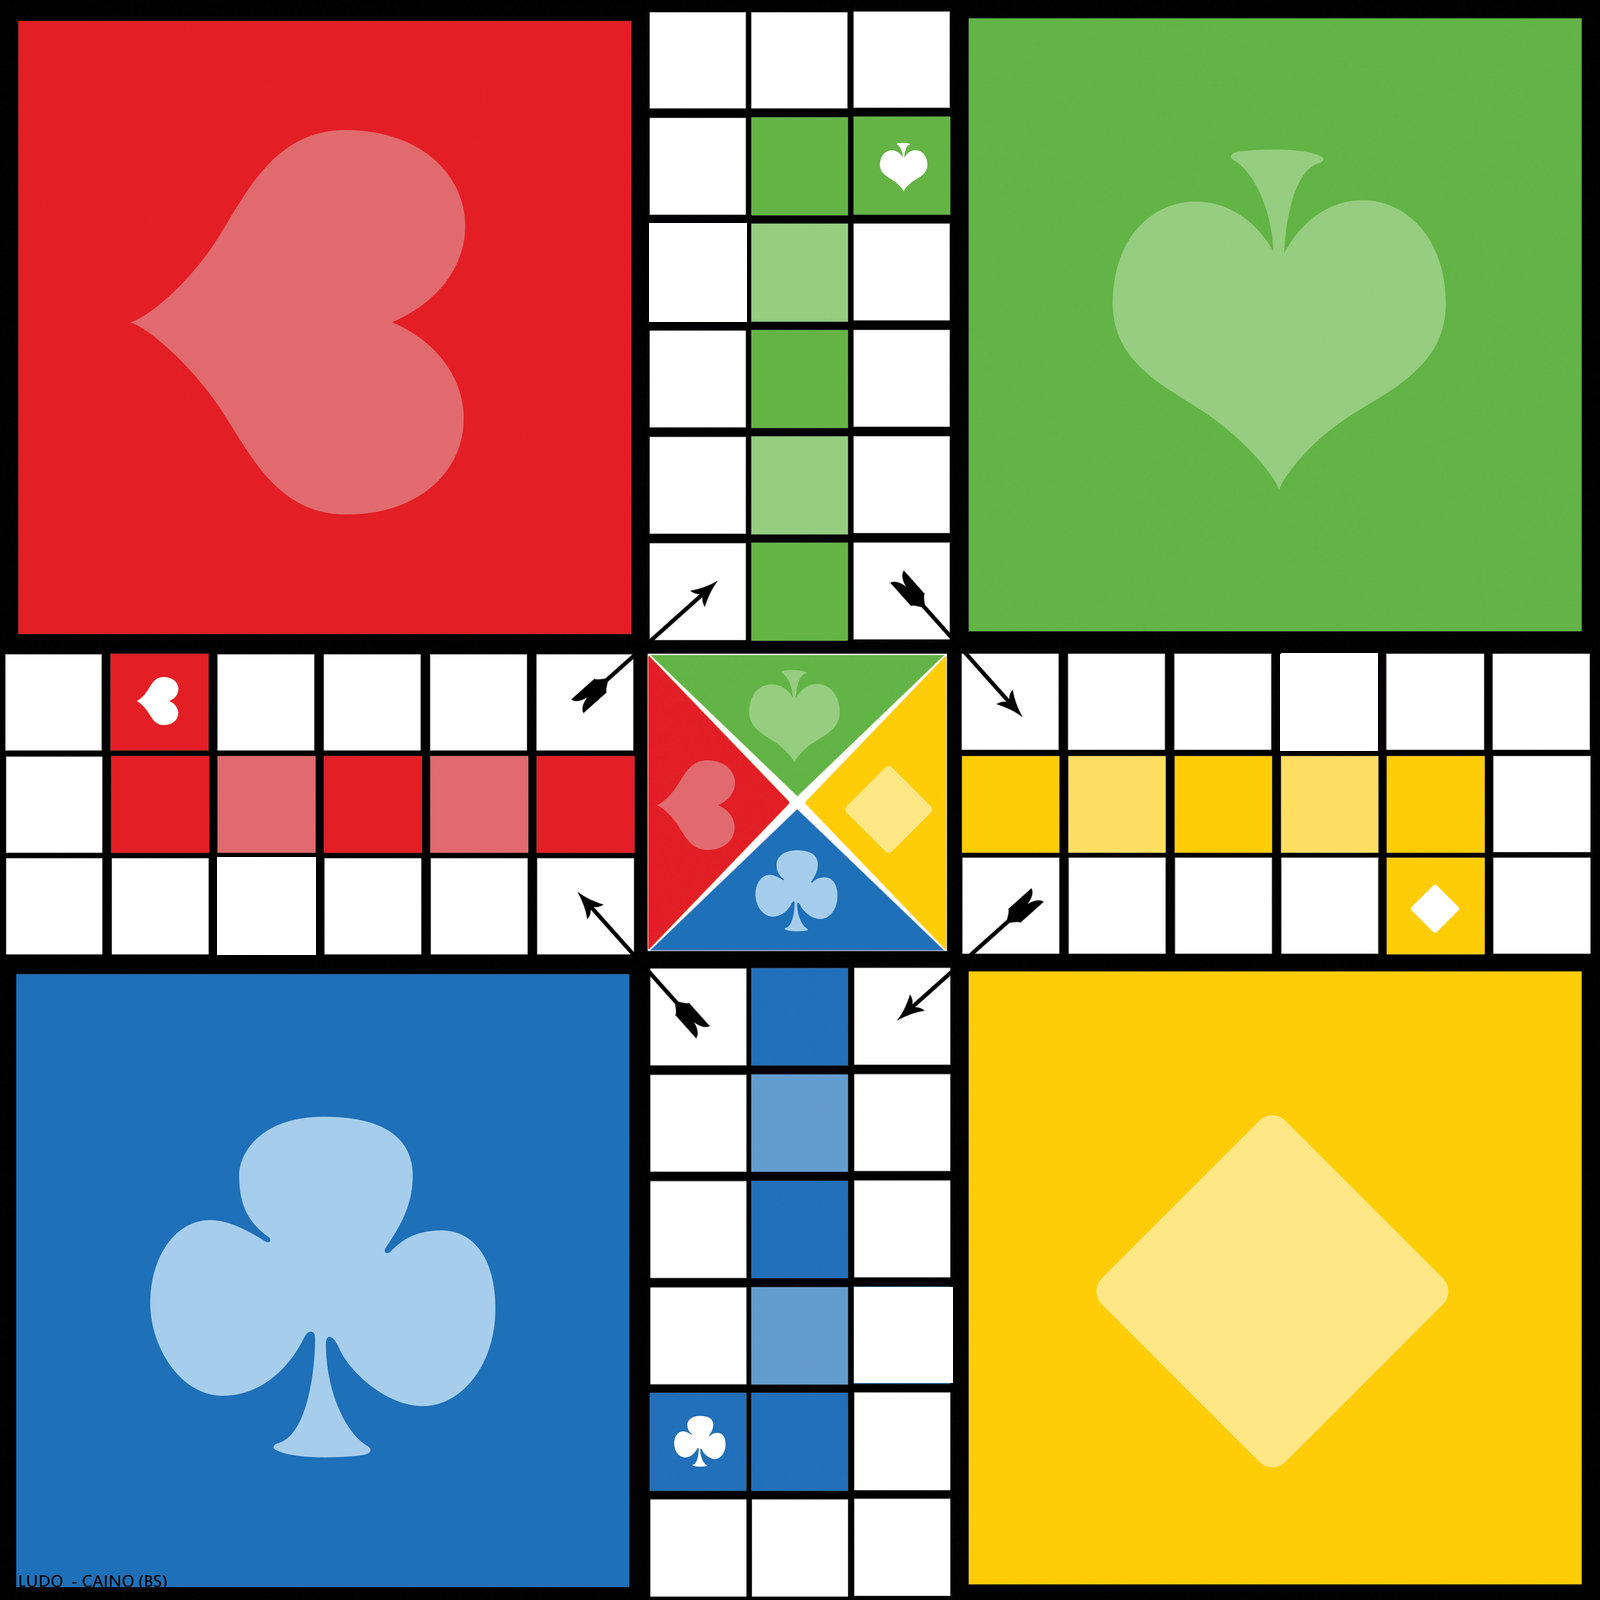
\includegraphics[width = 6cm]{ludobrett.png}}

\begin{document}

\frontmatter

\maketitle

\section*{Forord}

Ludøl er et fantastisk spill, og hovedforfatter av dette dokumentet har spilt 2
ganger, vært coach 2 ganger, og dømt mer enn en håndfull parti. Dersom det
gjennomføres riktig, er det en magisk opplevelse både å se på, dømme, coache
og spille.  

Ludøl krever dog endel forberedelse av arrangørene, spillerne, coaches og
dommer. Det har skjedd at spillere har blitt sendt med ambulanse til sykehuset,
og dette er noe en for all del vil unngå. Siden dette spillet -- uheldigvis --
ikke spilles hver uke, er denne håndboken et forsøk på en blanding av
styringsdokument, erfaringsoverføring og råd. Dersom du bare ønsker et raskt
eksempel på spillets gang se \cref{sec:forstegangs-dommer}. Dokumentet er noe
langt, så du trenger bare å lese de delene som er relevant for deg.

Først følger de vanlige ludo reglene, deretter ludøl reglene i sin helhet, og
tilslutt noen vanlige hus-regler. Dernest informeres det om hva som kreves for
å arrangere spillet, også følger kapitlene til spiller, coach og dommer. Disse
introduseres med en kort anekdote, før det kommer råd og tips. Hvert kapitel
avsluttes med \emph{satans råd} som er humoristiske råd en absolutt ikke burde
følge, men er alle basert på ekte hendelser.

\Cref{fig:maslows-ludol} viser regel-hierarkiet en vanligvis følger i ludøl. I
bunnen finner vi ludo reglene som alt bygges på. Disse reglene overskrives av
alle reglene over. Slik at Ludøl-reglene har prioritet over Ludo reglene,
Hus-reglene har prioritet over Ludøl-reglene også videre. På toppen finner vi
\cref{par:dommer}, som sier at dommer etter eget skjønn kan fravike fra alle
regler i pyramiden.

\begin{figure}[htbp!]
  \centering
  \includestandalone{./img/maslows-ludol-pyramid}
  \caption{}
  \label{fig:maslows-ludol}
\end{figure}

\tableofcontents

\mainmatter

\chapter{Ludo}

\section{Historie}

Patchesi fikk i 1795 for første gang et engelsk derivat da John Jaques \& Son
begynte å produsere det. Denne varianten var i bruk frem til 1920-årene[2].
Ludo, som kom i 1896, er en sterkt forenklet og mer barnevennlig versjon av
Patchesi. Spilleveiene er klarere fargemarkert og dessuten indisert med piler.
En større forskjell fra Patchesi er at man ved Ludo flytter brikkene med klokka.
Dermed ble Ludo det første Pachisi-derivatet som endret den opprinnelige
bevegelsesretningen.

\section{Regler} Reglene under er de opprinnelige ludo-reglene. De reglene
som overstyres av ludøl-reglene er streket ut, mens reglene i kursiv er regler
som er overstyres av husreglene.

\begin{ludo}
   
  \item \label{sec:ludo} Hver spiller starter med 4 brikker, i hver sin bås (blå, gul, rød og
    grønn).
     
  \item \sout{Målet med spillet er å være den første til å få alle brikkene sine
    i målet (med samme farge som brikkene og båsen).} Se \cref{par:avsluttes}.

  \item Brikkene flyttes fra båsen til målet ved at de først settes i spill og
    plasseres på spillerens frifelt, deretter flyttes de ved hjelp av terningkast
    med klokken på de hvite feltene rundt spillebrettet. \emph{Når en brikke er
    flyttet gjennom hele banen og står under den fargede midtrekken som leder opp
    til ens eget mål i midten, flyttes brikken oppover de fargede feltene mot
    mål.}\footnote{Overskrives av \cref{par:hus-hjem}}. 
   
  \item \emph{Den som har de røde brikkene begynner , deretter de gule , de blå og til
    slutt de grønne.}\footnote{Overskrides av \cref{par:hus-start}.}
   
  \item \label{para:ludo:seks} \sout{Når og bare når en spiller kaster seks
    ($6$), så kan en brikke flyttes ut av båsen og settes i
    spill.} [overskrides av Røros-konvensjonen, se \cref{par:roros}.]
    Når en spiller kaster $N$ ($1$ - $6$) på terningen, og har brikker i
    spill, så kan han flytte en brikke som allerede er i spill $N$ felt fremover.
   
  \item Når en spiller ikke har noen brikker i spill, har han opp til tre forsøk
    på å kaste seks ($6$) og dermed få en brikke i spill. Dette gjelder både dersom
    spilleren har alle fire brikker i startfeltet og når en eller flere er i mål.
   
  \item Når en spiller kaster seks ($6$) og har gjort sitt trekk, så får han et
    nytt kast og kan gjøre et trekk til.
   
  \item Feltet utenfor startbåsen er frifelt for brikker av samme farge. Stripen
    inn mot mål er også frie, da ingen andre brikker kan bevege seg på de feltene.
   
  \item Dersom en spillers brikke lander på et felt der en motspiller brikke
    står fra før, blir motspillerens brikke slått inn, tilbake til båsen. Dette
    gjelder ikke hvis motspillerens brikke står på sitt frifelt, \emph{eller hvis
    brikken flyttes videre i samme omgang etter at det har vært kastet
    6}.\footnote{red.adm, vent er dette en ting? Aldri spilt med den reglen
    hvertfall.} En kan likevel flytte videre fra eget frifelt i samme omgang dersom
    en motspiller brikke slås inn der.
   
  \item \sout{Dersom en spillers brikke lander på et felt der en egen brikke
    står fra før, danner disse brikkene en sperre for motspilleres brikker slik at
    de ikke kan passere. To brikker på samme felt kan heller ikke slås inn. Det
    samme gjelder ved tre eller fire brikker på samme felt. Brikkene må flyttes
    videre enkeltvis.} [Overstyres av \cref{par:sperre}.]
   
  \item \emph{Eksakt kast kreves for å få en brikke i mål.} \footnote{Denne
    regelen overskrives indirekte av \cref{par:hus-hjem}, siden det ikke er
    mulig å få brikker i mål.}
   
  \item \sout{Vinneren er den første spilleren som får alle sine brikker i mål.}
    [Overstyres av \cref{par:avsluttes}.]
  
  \item \sout{Dersom det står to ($2$) eller flere står på samme felt så er det
    sperre. Du kan ikke flytte forbi disse eller slå de ut.} [Se \cref{par:sperre}].
\end{ludo}

\chapter{Ludøl}

\section{Historie}

Ludo fikk 17. oktober 1987 for første gang en norsk derivat da Christian Larsen
\& Geir Wagbø begynte å konsumere øl. Denne varianten var i bruk frem til
1990-årene[2]. Ludøl, som kom i 1991, er en sterkt forvansket og mindre
barnevennlig versjon av Ludo. Spilleveiene er klarere fargemarkert og dessuten
indisert med piler. En større forskjell fra Ludo er at man ved Ludøl flytter
glass og ikke brikker med klokka. Dermed ble Ludøl det første Ludo-derivatet som
endret spillets opprinnelige hensikt, og det ble i stedet ett meningsfylt
fritidstilbud for studenter landet rundt.

\begin{figure}[htbp!]
  \centering
  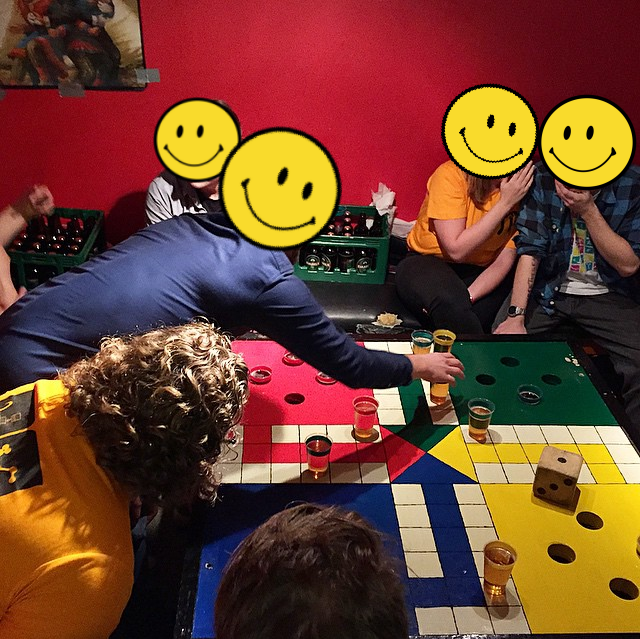
\includegraphics[width=0.65\textwidth]{ludol-live} 
  \caption{Ludøl i aksjon med anonymiserte spillere.}
  \label{fig:ludol-live}
\end{figure}

\newpage

\section{Regler} 

\begin{ludol}

\item \label{sec:ludol} Spillets navn er \textsc{LUDØL}.

\item Spillets hensikt er å gi studenter et meningsfyllt fritidstilbud.

\item Spillet skal kun ha én dommer. Hvis spillet etterhvert skulle utvikle seg
  mot kaotiske tilstander og anarki, eller hvis dommeren av andre årsaker skulle
  miste kontrollen, kan denne utpeke to linjedommere som hjelpemannskap.

\item \label{par:forkunnskaper} Dommeren plikter på forhånd å gjøre seg kjent med Ludøl-spillets
  paragrafer og bør selv ha gjennomgått Ludøl's prøvelser.

\item \label{par:dommer} Dommeren kan etter eget skjønn avvike fra disse paragrafer.

\item Spillet skal ha maksimalt fire ($4$) deltakere.

\item To eller flere deltakere kan ikke dele samme farge.

\item En deltaker kan godt spille flere farger.

\item Spillet følger alminnelige ludo-regler med de utvidelser som er nedfelt i
  disse paragrafer.

\item Deltakerne kaster om å begynne. Spilleren med høyest terningkast starter
  og blir tildelt bokstav $A$, spilleren til venstre blir tildelt $B$, nestemann
  $C$ osv. For å få brikkene hjem, må de havne på riktig felt i
  avslutningsfeltet.

\item Som brikker benyttes glass som (mens de er i aktivt spill) skal være fylt
  med edelt Pilsner-Øl (\SI{4.5}{\percent}) eller sterkere drikke.

\item Idet et glass blir slått hjem, skal spilleren som eier glasset tømme dette
  innen $10$ sekunder. De andre deltakerne plikter å telle høyt og tydelig fra
  $10$ til $0$.

\item \label{par:sperre} En spiller kan sperre andre fra å passere ved å ha to eller fire glass
  stående på samme felt. Merk at tre glass \emph{ikke} sperrer. Ved hjemslåing
  må alle glass tømmes. En spiller kan fritt passere sin egen sperre.

\item En spiller kan ikke slås hjem når han/hun står i sitt
  \textquote{startfelt}.

\item \label{par:roros} %Label skaper ankerpunkt til refferanser
  Røros-konvensjonen gjelder under alle normale kast. For de uinvidde betyr
  dette at spilleren som kastrer terningen fritt kan velge om han/hun ønsker å
  benytte oversiden eller undersiden av terningen.

  % Presser inn en ny side, og lar den nye siden begynne 2.38cm høyere opp enn
  % normalt. Nødvendig for å få det på to sider.

 \ifnothandbok{\newpage %
  \vspace*{-1.38cm}} 
  \thispagestyle{empty} % Fjerner sidetall

\item \label{par:roros-2} %Cref gir stor bokstav til refferanser. Henviser til røross-paragrafen.
  \Cref{par:roros} trer ikke i kraft under følgende omstendigheter:

  \begin{ludol}

  \item Ved innledende kast om hvilken spiller som skal begynne.

  \item I det en brikke befinner seg i, eller flyttes inn i avslutningsfeltet.
    Merk at \cref{par:sekser-regelen} har prioritet over denne paragrafen.
    \ifhandbok{Overskrides av husregel 19}.

  \end{ludol}

\item Dommeren kan etter eget skjønn tildele en eller flere spillere
  straffepils. Det anbefales på det sterkeste at dette gjøres ved følgende
  tilfeller:

  \begin{ludol}

  \item En spiller kaster terningen slik at den faller på gulvet.

  \item Ved alle tilfeller der en spiller er ansvarlig for ødsling av edelt
    drikke.

  \item Hvis en spiller unnlater å benytte anledningen til å slå hjem en brikke
    av annen farge.

  \item Hvis en spiller ikke er tilstede idet det er dennes tur til å kaste
    terningen og nedtelling fra $10$ til $0$ er utført av de andre deltakerne.
    Dette medfører at man bør være rask under eventuelle toalettbesøk.

  \item Hvis en spiller er tilstede, men (etter nedtelling) likevel ikke er klar
    over at det hans/hennes tur til å kaste terningen.

  \item Ved ethvert forsøk på å kverulere over dommerens avgjørelse.

  \item Hvis en spiller viser liten evne til å vite hvilken farge som er ens
    egen.

  \item \label{subpar:passivt} Ved forsøk på passivt spill.

  \end{ludol}

\item \label{par:sekser-regelen} En spiller kan i henhold til \cref{par:roros}
  velge om han/hun vil benytte terningen som en éner ($1$) eller sekser ($6$)
  hvis et av disse tallene oppnås under kast. Velger spilleren én ($1$), flyttes
  glasset ett felt framover, og spilleren får ikke ekstra kast (han/hun kan
  imidlertid risikere å bli idømt straffepils i henhold til
  \cref{subpar:passivt}). Hvis spilleren velger å benytte terningen som en
  sekser ($6$), flyttes glasset seks felter fram (eller et nytt glass flyttes
  \textquote{ut}), og spilleren får ekstrakast. Fra og med tredje kast, må
  spilleren imidlertid velge seks ($6$) hvis terningen viser én ($1$) eller seks
  ($6$), og spilleren idømmes i tillegg én straffepils for hver sekser (éner)
  fra og med den tredje.

\item \label{par:offentliggjore} Den som for tredje gang ser seg nødt til å
  offentliggjøre sin middag, diskvalifiseres.

\item \label{par:avsluttes}. Spillet avsluttes når:

  \begin{ludol}

  \item \label{subpar:hjem} En spiller har fått alle sine glass hjem.

  \item \label{subpar:tom} I det dommeren har skjenket all drikke.
    \ifhandbok{ALLAH AHKBAR} 

  \item \label{subpar:middag} Alle untatt én er diskvalifisert i henhold til
    \cref{par:offentliggjore}.

  \end{ludol}

\item Hvis spillet er avsluttet i henhold til \cref{subpar:hjem}. eller
  \cref{subpar:middag}, er vinneren den person som fikk alle sine glass
  hjem/ikke ble diskvalifisert. Hvis spillet er avsluttet i henhold til
  \cref{subpar:tom}, telles alle glass sin avstand (i felter) fra startfeltet.
  For de glass som ennå er hjemme, trekkes det ti ($10$) felter fra. For de
  glass som allerede er kommet inn, legges ti ($10$) felter til summen. Vinneren
  er den spilleren som oppnår høyest sum.

\item Ved avslutning kan spillerne tømme sine respektive glass hvis de ønsker
  dette.

\item Hvis spillet er avsluttet i henhold til \cref{subpar:hjem} eller
  \ref{subpar:middag}, blir vinneren tilkjent resten av kassen, såfremt den
  tømmes i løpet av kvelden.

\end{ludol}


\chapter{Husregler}

Ludøl er over 30 år gammelt, og forståelig nok har reglene endret seg noe på den
tiden. Dette kapitelet er et forsøk på å skrive i stein de reglene som det har
blitt spilt med i praksis, men så langt bare har vandret på folkemunne.

\begin{hus}
\item \label{sec:hus} Det anbefales på det sterkeste å ha en til to
  linjedommere.

\item Coach plikter seg til å passe på sin spiller fra og med spiller setter seg
  ned ved bordet til spiller ligger hjemme i sengen sin.

\item Coach skal skrive telefonnummeret sitt og adressen til spiller på armen
  til sin spiller.

  \item Coach plikter seg til å kaste inn håndkleet dersom spiller virker ute av
    form til å fortsette. 

\item \label{sec:hus-coach} Hver spiller skal ha minst en coach, og kan og
  gjerne ansette en person til å åpne og fylle opp glassene med pils (øl-ape).

  \item Det er øl-apens ansvar å tømme bøtten, mens bøtten tommes overtar coach
    midlertidig ansvaret som øl-ape.
    
\item \label{par:hus-start} Deltakerne kaster om å begynne. Spilleren med høyest
  terningkast starter og får velge farge. Deretter får spilleren med nest høyest
  terningkast velge farge osv. Dersom to spillere kaster likt blir det omkast
  til en spiller triller høyest.
    
\item \label{par:hus-hjem} Det er ikke mulig å få brikkene i mål. Dersom en
  brikke har gått en runde rundt brettet fortsetter den å gå rundt og
  \emph{ikke} opp de fargede feltene mot mål.
    
\item Dommer kan etter eget skjønn tildele en eller flere spillere skåler. Det
  anbefales på det sterkeste at dette gjøres ved følgende tilfeller:
    
    \begin{hus}
    \item Ved spillestart for å feire ett meningsfylt fritidstilbud.
      
    \item Når en spiller har klart å gå en runde rundt bordet.
      
    \item Når noen ser seg nødt til å offentliggjøre sin middag.
    \end{hus}
      
  \item \label{par:hus-avsluttes} Spillet avsluttes når alle unntatt én har sett
    seg nødt til å offentliggjøre sin middag tre ganger.
\end{hus}


\chapter{Forberedelse}

Under følger en kort liste med nødvendig utstyr før spillet settes igang.

\begin{enumerate}

  \item \textbf{Svært ludobrett}.

  \item \SI{200}{\ml} \textbf{glass}.

    Dette er et absolutt krav. Spillet KAN IKKE og MÅ IKKE spilles med hverken
    større eller mindre glass. Mindre glass gjør at spillerne ikke drikker raskt
    nok til å vise middagen sin før det blir farlig. Mens større glass gjør det
    umulig å fullføre glasset på 10 sekunder.

  \item \textbf{Elektrikkertape} eller \textbf{fargede glass}.

    Realfagskjelleren har lenge brukt elektrikkertape for å markere glassene.
    og dette er en flott måte å skille glassene til hver spiller fra hverandre.
    Elektrikertapen fra Biltema holder ca til 15 glass i hver farge. 
    Undertegnede har vært dommer når det har blitt spilt med umerkede glass, og
    dette har vært kaos uten like.

    Alternativt kan en bruke fargede glass som Abakus lenge har brukt. Det
    viktigste er at det er tydelig forskjell rød, grønn, gul og blå sine glass,
    samt at en enkelt skal se hvor fulle glassene skal være.

  \item \textbf{5 Bøtter}.

    Skaff en spy bøtte til hver spiller. Når en spiller er ferdig å spy, får
    spilleren reserve bøtta mens coach tømmer den andre. Dette er slik at
    spillet ikke skal stoppe for lenge opp.

    Ikke be flere deltagere dele samme bøtte, og skaff nye bøtter ved jevne
    mellomrom. Undertegnede har og vært med på at det har vært brukt svært gamle
    bøtter med hull i. Ikke veldig kos når gulvet fylles
    med en blanding nuddler og leskende Dahls.

  \item \textbf{Terning}.

    Terningen bør være stor og vektet IKKE bruk en Yahtzee terning! Mange av
    reglene i Ludøl dreier seg nemlig om terningen. Dersom terningen havnet
    utenfor bordet, dersom terningen skumper borti glass slik det søles, eller
    dersom terningen viser for mange seksere (3) på rad skal det drikkes. De to
    første punktene skjer langt oftere med en mongostor terning. Mens det siste
    punktet kan fikses ved å vekte terningen. F.eks. en stor Gummi-terning
    fungerer ypperlig, den spretter ut av bordet ofte.

  \item \textbf{Tusj!}

    Spillerne SKAL skrive adressen sin på armen før spillet start. Dette er for å
    forsikre oss om at spilleren kommer seg hvem tilslutt.

  \item \textbf{Mikrofon}

    Spillet kan ofte utarte seg til kaotiske tilstander. Dersom det står 100
    mennesker i bakgrunnen og prater, kan det være umulig for spillere og ikke minst
    publikum å høre dommer. Utestemmen varer bare så lenge, så en god mikron (eller
    kanskje megafon? :p) kan komme godt med.

  \item Lokalet med \textbf{toalett nærme} spillebordet. Bøtter må tømmes.

  \item \textbf{Tørkepapir}. Masse tørkepapir.

  \item \textbf{4 flaskeåpnere}+.

  \item 4/5 kasser Dahls.

    Det pleier å gå alt mellom $3 \cdot 24 \cdot 0.33l \approx 24 $ til $5 \cdot 24
    \cdot 0.33 = 40l$ totalt. Anbefales å regne litt over 4 kasser for å være trygg.

\end{enumerate}

\begin{figure}
\end{figure}

\begin{figure}
    \centering
    \begin{subfigure}[b]{0.45\textwidth}
      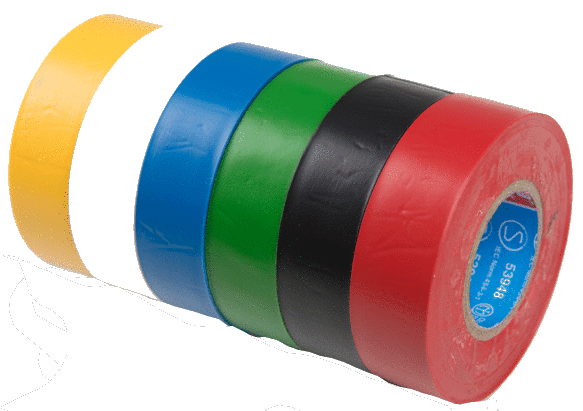
\includegraphics[scale=0.2]{sportstape.png}
        \caption{Elektrikkertape}
        \label{fig:utstyr-terning}
    \end{subfigure}
    ~ %add desired spacing between images, e. g. ~, \quad, \qquad, \hfill etc. 
      %(or a blank line to force the subfigure onto a new line)
    \begin{subfigure}[b]{0.45\textwidth}
        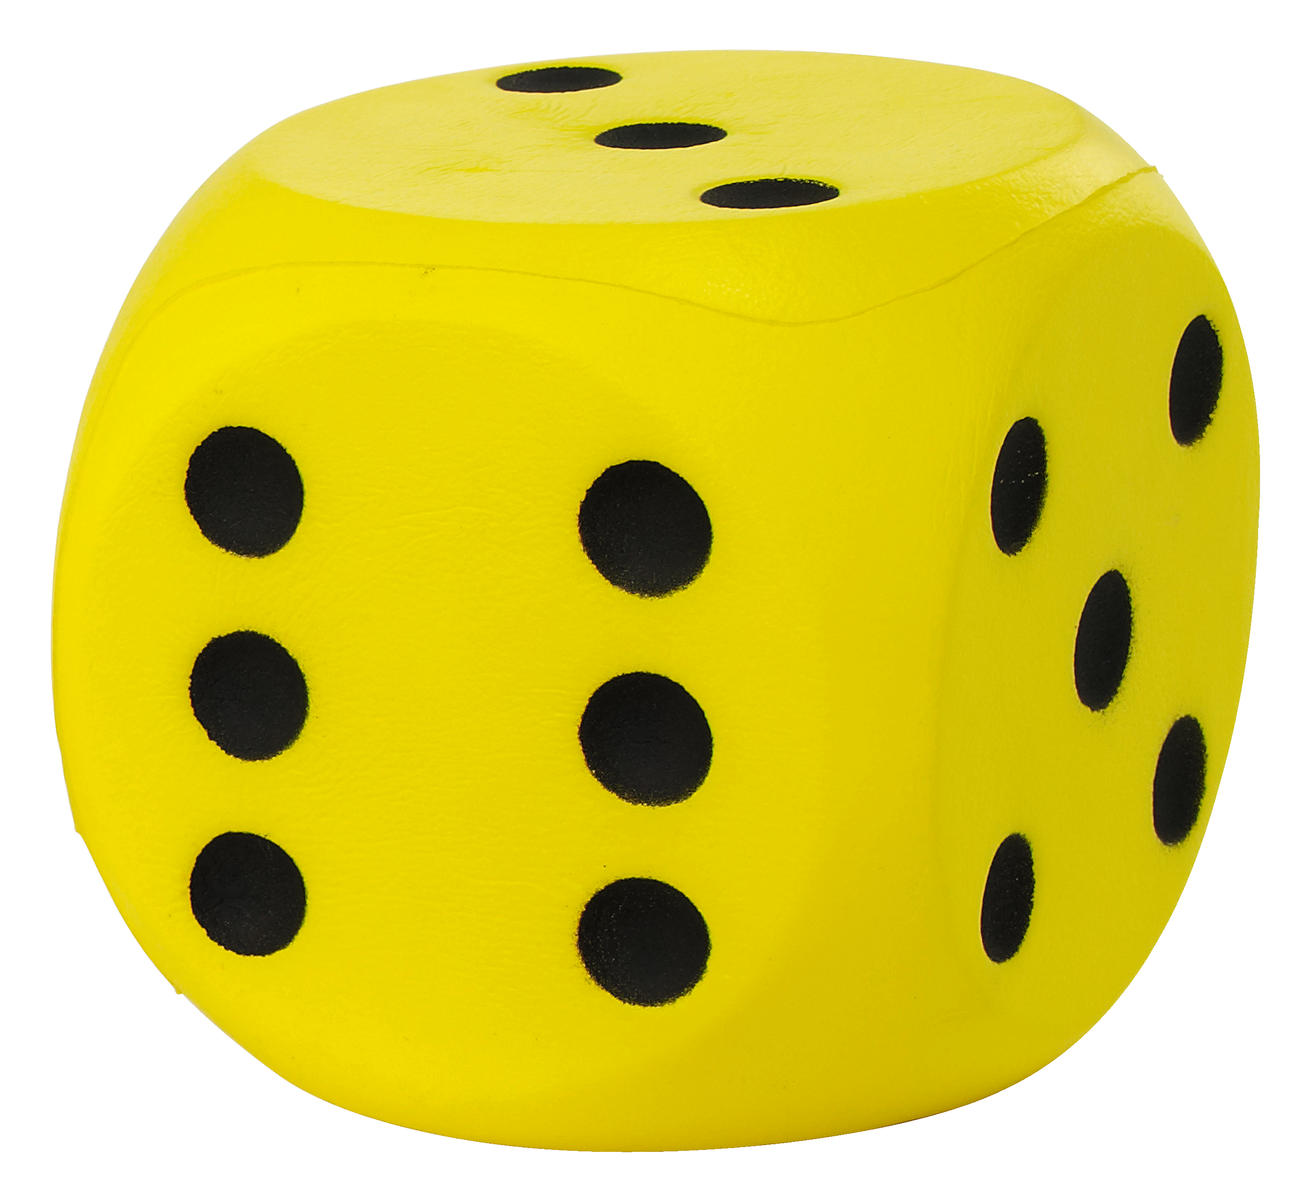
\includegraphics[scale=0.1]{terning.jpg}
        \caption{Gummi-terning}
        \label{fig:utstyr-terning}
    \end{subfigure}
    \caption{Utstyr}\label{fig:utstyr}
\end{figure}


\chapter{For Spiller}

\epigraph{Mindset: \say{hvordan fucke seg selv mest mulig?} Med mindre du kan ta
  noen andre}{\textit{Førstegangsspiller}}

Det aller aller viktigste å huske er at du taper etter tre spy, se
\cref{par:offentliggjore}. Vinneren er den som ikke har spydd 3 ganger, jamfør
\cref{par:hus-avsluttes}. Dersom du veier lite, eller ikke er vant med å
konsumere store mengder øl, frarådes det sterkt å spille. Det samme dersom du
ikke har sett spillet før. Men før strategier og flere advarsler gis tas en kort
fortelling.

\blockquote[Brage Sæth]{%
  Som mangeårig fan av dette edle spillet er det godt å vite at det kommer
  etterfølgere som vil gå i de samme baner som det jeg selv har gjort. Det er
  helt vanlig å kjenne sommerfugler i magen før man skal spille, men husk på
  disse kommer mest sannsynlig til å ta følge med middagen under spillet. Dersom
  du synes øl er godt, er det ingenting som hindrer deg i å spille, ikke la
  frykten stå i veien for at du får et meningsfullt fritidstilbud. Noe av det
  viktigste ved spillet er at man har en coach som du stoler på og som virkelig
  vet hva Ludøl går ut på. Jeg husker selv den første gangen jeg skulle spille
  dette edle spillet, hverken jeg eller min coach hadde mye peiling på hva som
  ventet oss. Hva reglene var og hvordan en burde spille. Det ble ett hardt møte
  med virkeligheten, men det var verdt det. Jeg fikk se og føle på noe av det
  vakreste Trondheim har å by på. Det oppstår også et kameraderi mellom
  spillerne, vi var alle der for gjøre opp om ære og berømmelse, og bare ha en
  koselig kveld.}


\section{Råd og tips}

Det viktigste som spiller er å ansette ett godt støtteapparat rundt deg. Dette
involverer en dyktig coach, en øl-ape se \cref{sec:ol-ape} og om mulig noen som
kan kjøre deg hjem. Det beste er å ha en coach som har sett spillet før, enda
bedre spilt eller best ha dømt. Velg noen du kjenner godt og kan stole på passer
på deg etter endt spill. Det anbefales å spise en solid frokost før du skal
spille, samt en liten lunsj.

Du er bøtta. Hva betyr dette? En flink spiller skal kunne drikke mye, og
utelukkende følge rådene til coach nøye. Du kan gjerne komme med forslag til
trekk til coach, men det er til syvende og sist coach som burde bestemme. Jobben
din som spiller burde med andre bare være å drikke, men ikke for mye. Med andre
ord minimer feilene dine, ikke krangle med dommer, kaste terningen utenfor
bordet, trille for mange seksere, søle alkohol osv. Mens coachen din skal passe
på at du ikke spiller passivt. Basert på tidligere erfaring kan det være lurt å
ta en taktisk spy, etter ca 7-10 øl (0.33l), alt ettersom. Spy mest mulig når du
spyr, her er det fingrene i halsen til du smaker galle. Stort sett får du spy så
lenge du vil, så ta tiden til etterretning. Det samme er når du skal drikke,
bruk de 10 sekundene. Det er ikke vits å sluke glasset på 4 sekunder dersom du
ender opp med å søle. \medskip

\noindent
Dersom du ønsker å vinne kan du fortsette å lese her, samt ta quizen på side
\pageref{chap:quiz}.
\begin{enumerate}
    
  \item For de beste
vinnersjansene burde en spille en liten runde ludøl uten drikking på
    forhånd for å virkelig lære seg ludo, samt hvordan ikke spille passivt.
    
  \item Flatrulling. Dette betyr at du legger terningen i håndflaten, og bare
    vipper den ut slik at den lander på det tallet du ønsker. Avhengig av dommer
    kan en gjøre dette mye eller lite, og det er ofte at dette straffes med
    drikking. Men dersom du ser ditt snitt til å eksempelvis slå ut tre av
    motstandernes glass dersom du flatruller, er det bare å kjøre på.
    
  \item Minimer tapene dine. Anta at du spiller med to farger, og har trillet
    slik at du enten kan flytte fremover, eller slå ut ditt eget glass. Dersom
    du slår ut ditt eget glass må du drikke, men dersom du flytter frem må du også
    drikke (passivt å ikke slå ut seg selv.). Men, her burde en virkelig ikke slå
    ut seg selv. Dersom du må drikke uansett er det bedre å flytte frem, slik
    at en kan jage andre, i stedet for å måtte slå ut seg selv.
    
  \item Ikke vær for hyggelig med de du spiller mot. Det å le, smile, og skåle
    er helt innafor, men ikke si ifra om hvem sin tur det er, eller gi terningen
    til neste spiller. Dette må de passe på selv, og det kan føre til at de må
    drikke, uten at du blir tatt for passivt spill. 
\end{enumerate}


\section{Satans Råd}

\begin{enumerate}
	\item Det er oppskrytt å kunne reglene i ludo.
    
	\item Alltid spis en stor middag. Spis gjerne flere middager, og prøv å bland
    mest mulig forskjellig. Nudler, tunfisk, egg og lasagne er en klassiker. Dunsten av
    ditt eget oppkast vil få motstanderen til å spy som en
    flodhest.$\!$\footnote{Virker ikke dette er det bare å sikte på bordet og ikke
    bøtten neste gang du spyr.}
    
  \item Gjerne ta et vorspiel eller to før spillet og konsumer en hel kasse
    der. En kan og øke alkoholtoleransen ved å være ute på whisky-fylla dagen før.
    
  \item Jenter elsker personer som nettopp har spilt ludøl, prøv gjerne å
    sjekke opp flest mulig like etterpå. Spesielt din kvinnelige coach som
    for 10 min siden bar deg sammen med typen sin inn på do for å spy.

  \item Dommeren er den som kan minst i spillet, gjerne forklar dommeren
    hvordan ting bør dømmes. Dommeren liker en god krangel.
    
  \item Det anbefales å spille med iskald Tuborg samt å åpne flaskene rett før
    konsumering.
    
  \item Prøv gjerne å telle mens du drikker. 
    
  \item Dopauser er for pingler. En flaske Baccardi Razz eller din egen bøtte
    fungerer utmerket som toalett.
    
  \item Fukt gjerne strupen med Gin eller andre drinker på siden.
    
  \item Har du problemer med å spy, prøv å stikk skaftet på en stekepanne langt ned i ganen.

  \item Det å dra på byen etter å ha spilt er en ypperlig idé

  \item Dersom du av en eller annen merkelig grunn har blitt kjørt hjem i taxi,
    bare gjem deg i buskene til han har kjørt. Da kan du snike deg opp på
    kjelleren igjen selv om det tok deg 3 timer å sjangle dit.
\end{enumerate}


\chapter{For Coach}

\epigraph{``Look at me. I am the captain now!''}{Coach til vrang spiller.}

Den aller viktigste jobber til coach er å passe på deltaker fra den setter seg
ved bordet, til han/hun ligger i sengen. Samt å heller kaste inn håndkleet for
tidlig enn for seint. Det er pinlig å måtte ta en tur på sykehuset, så unngå
dette. Som coach er det og svært viktig å huske at det er du som faktisk
spiller. Mens spilleren triller og drikker, er det du som coach som burde ta
elle beslutningene om hvor og når det burde flyttes, eller drikkes. Les reglene
\emph{nøye} det er pinlig dersom spiller må drikke fordi ingen av dere kan
alminnelige ludo-regler. Se quizen bakerst på \pageref{chap:quiz}. Under er en
kort liste med hint og tips til å være en god coach.

\begin{enumerate}
  \item Det er din oppgave å kaste inn håndkleet før spilleren blir altfor full.
    Dersom spilleren din har blitt for full, og det er vanskelig å få i
    spilleren vann, prøv og tell ned fra 10. 
    \item Følg LATTERLIG nøye med på spillet. Både når det er din spillers tur,
    men også når de andre spillerne spiller. 
  \item Selv om du bare ser bort fra bordet i 30 sekunder, kan det skjer
    mye som gjør at spilleren din må drikke. Det anbefales på det sterkeste å
    ansette en øl-ape, slik at du kan utelukkende konsentrere deg om brettet. 
  \item Følg nøye med på hvem sin tur det er. Det skjer konstant at spillere må
    drikke fordi coach glemmer hvem sin tur det er.
  \item Anta at noen har spydd, og din spiller tar en sympatipils. Da skjer det
    ofte at spiller setter ned glasset på feil felt. Derfor må du passe på hvor
    alle glassene til spilleren din står, til enhver tid. Dette kan minimeres
    ved å be spiller ALLTID drikke fra huset / båsen sin om mulig.
  \item Hindre spilleren din fra å drikke unødvendig Det har skjedd at spiller
    A har glemt at han allerede har gjort turen sin, også gjør han turen sin
    igjen og da slår ut B. Coach til B burde da vite at A har gjort en feil, og
    hindre sin spiller B i å drikke. Dette er bare ett av mange eksempler på
    hvorfor coach må følge med.
  \item Dommer endrer ofte på reglene. Enten i form av at deler av brettet ikke
    lengre spilles på, frifelt og blokader oppheves, eller at glassene begynner
    i frifeltene. Det er din oppgave som coach og huske på regelendringene.
  \item Nesten likt som punktet over er det viktig å lese dommer. Dette betyr
    IKKE å spørre dommer om hvilket trekk som er best, eller prøve å lese
    ansiktsuttrykkene til dommer når en gjør trekk.

    I stedet betyr det å legge merke til hvilke vaner dommer har, hva dommer
    dømmer hardt på og hva han ser igjennom fingrene på. Kanskje dommer ikke
    dømmer så hardt på søling, eller kanskje han ser igjennom fingrene på
    flatrulling dersom en spiller veldig aggressivt
  \item Noen ganger er alle trekkene du kan gjøre passive. Dette må du bare
    godta, og da velge det trekket som gjør at du i neste runde kan slå ut de
    andre spillerne (jage).
\end{enumerate}

\section{Øl-ape}
\label{sec:ol-ape}

En god øl-ape søler ikke når det helles, og åpner øl i god tid før det trengs.
Ofte er det mye kullsyre som knekker spillerne, og ved å la ølen være åpen i
noen minutter minker man dette problemet noe. Tilsvarende burde en ikke spille
med iskald pils, da dette er forferdelig å chugge. Merk at spillerne må drikke
dersom glassene ikke er fylt opp skikkelig. Dette betyr at du må minimere
mengde skum i glassene. Det anbefales derfor om du får lov av dommer å sette
glasset svært på skrå mens en heller. 


\section{Satans Råd}

\begin{enumerate}
  \item Dersom spilleren din har spilt kvalik dagen før O'store og deretter
    dro på whisky-fylla, er det ikke
    vesentlig at du har riktig telefonnummer til spilleren din. Hva er det
    verste som kan skje, at du må spille i stedet?
    
  \item Det er ikke nødvendig å sitte ved siden av spiller. Gjerne vandre litt
    rundt i rommet, og kjøpt en øl fra baren. Spilleren klarer seg sikkert på egenhånd.
    
  \item Dersom spilleren din ønsker å spille med to farger, når alle andre
    spiller med en, si ja. Alt annet ville vært passivt spill.

  \item Dersom spilleren din får kalde føtter to minutter før spillestart er det
    bare å bytte plass. Hvem legger merke til sånt?

  \item Når spilleren din spyr er dette en ypperlig anledning til å ta frem
    matboksen sin å spise litt.

  \item Utstyr gjerne spilleren med vernebriller, refleksvest og hjelm. Brillene
    beskytter mot spy, mens hjelmen gjør at du kan slå spiller i hodet for dumme
    feil.

  \item Når spilleren din ryker ut anbefales det å trille vedkommende ut i en
    trillebår.

  \item Dersom spilleren din spør deg om en regel i ludo, le høyt av vedkommende
    og si ``vet du ikke det engang?''. Selvsagt må du ikke svare på spørsmålet.
\end{enumerate}


\chapter{For Dommer}

\epigraph{L'état c'est moi}{\textit{Fransk ludøldommer.}}

\blockquote[øistein Søvik]{%
  Første gang jeg var dommer var jeg svært nervøs, pulsen var høy og hjertet
  dundret i ørene mine. Jeg følte at jeg hadde et ansvar for spillerness helse
  og velvære. Kommer de til å høre på han lille fjotten der som ikke engang
  kunne ludo første gang han spilte? Heldigvis var spillernes og arrangørene
  enda mer urutinerte enn meg. De spurte om det holdt med 2 bøtter, om
  spillerne kunne spille med halvliter glass og om jeg tilfeldigvis hadde en
  terning. Spillerne var -- om mulig -- enda dårlige, de kunne hverken ludo
  eller ludøl, men det oppstod ett kameraderi mellom dem. Det var spillerne mot
  dommer, og selv om de visste at de ikke kunne vinne hadde de en magisk kveld.
  Da kunne jeg endelig slappe litt av, og selv om jeg i ettertid innså at jeg
  kunne vært enda strengere var det en magisk kveld for meg og. }


Den viktigste jobben til dommer er å være en kreativ, men rettferdig kuk. Du
skal passe på at deltagerne spyr før de får en kasse eller mer inn i blodet.
Det farligste er en for snill dommer, for da kan deltager-ene fort havne på
sykehuset. Normal spilletid for ludøl bør ligge mellom $1$ til $2$ timer alt
ettersom, men det er mer viktig å passe på formen til deltagerne. Dersom
spillerne ikke virker spesielt fulle er det ikke farlig om spillet varer litt
over $2$ timer, men dersom det er fare for liv og helse bør en enten
diskvalifisere spillerne eller øke tempoet betraktelig. Merk at det ikke er
alkoholen som får deltagerne til å spy, men stort volum og mye kullsyre på
liten tid. Tre glass på rad er ofte mye verre enn 6 glass fordelt jevnt over $2$
runder. Merk at en ikke trenger å stresse for mye over at spillerne skal drikke
konstant, en time er faktisk ganske lenge. Hold ett øye på klokka så går det
alltid fint. Såfremt du ikke dømmer finalen i O'store. 

Forkunnskapene en trenger for å stille som dommer er heldigvis enkle, du bare ha
spilt før. Se \cref{par:forkunnskaper}, merk at selv om det skrives
\emph{anbefalt} har det ikke skjedd på 10 år at noen er dommer uten og ha spilt
ludøl før. Det anbefales og å lese over de vanlige reglene i ludo, ta quizen på
side 4 for å sjekke hvordan det står til med forkunnskapene. Som dommer må du ha
en sterk rettferdighetssans, kunne ta raske avgjørelser, samt ha ett godt
overblikk, men kanskje viktigst av alt du må ikke være konfliktsky.

Det å dømme er en hard jobb, og det kan tidvis føles ut som en coacher fire
spillere samtidig. Det kan derfor anbefales på det sterkeste å ansatte to
linjedommere til jobben. Disse trenger ikke å ha sett spillet før, men bør har
gjort seg godt kjent med både ludo og ludøl reglene på forhånd. Det å f.eks
delegere en linjedommer til å utelukkende følge med på passivt spill, og en
annen til å følge med om glassene står riktig kan være lurt. 

\section{Førstegangs dommer} \label{sec:forstegangs-dommer} Dersom du skal
dømme og bare ønsker å følge en enkel fremgangsmåte kan du følge kulelisten
under. Merk at noe av sjarmen er å ha sin egen vri på dømmingen.
%
\begin{enumerate}
    \item Sjekk at deltagerne har skrevet adresse på armen og at coach og
    spillere har gjort seg kjent med reglene.
    
    \item Start med å be spillerne trille om hvem som skal starte. Høyest
    begynner, Røros-konvensjonen gjelder ikke her. Har du mulighet lar du den
    som triller høyest få bestemme farge, og dermed også
    bordplassering.\footnote{Taktisk i forhold til toalett og slikt.}
    
  \item Før spillet begynner må publikum lære å telle. Du velger da om
    spillerne skal skal tømme 1+(1), 2+(1), 3+(1) eller 4 glass. Tallet på
    slutten symboliserer en rolig skål som tas tilslutt og en ikke teller på.
    Når skålen er over starter den som trillet høyest.
    
  \item Del ut straffeslurker for passivt spill over en lav sko. Dersom spillere
    ikke aktivt utsetter seg selv for maksimal fare er det passivt.
    
  \item Etter \SI{20}{\m} be spillerne starte i startfeltet og ikke i båsen /
    huset.
    
  \item Dersom en spiller spyr utbringer de andre en sympati-skål. Coach har
    ansvar for å tømme bøtta før spillet fortsetter. Merk deg hvilke spiller som
    skal starte etter pausen. Dersom denne spilleren ikke vet det, må det
    drikkes.
    
  \item Etter \SI{40}{m} fjernes frifelt.
    
  \item Dersom en spiller går ut, kutt denne delen av brettet.
    
  \item Etter \SI{60}{m} fjern blokader. Merk nå at alle glassene som nå står i
    frifeltet ``plutselig'' kan slås ut når som helst.
    
  \item Dersom det er to spillere igjen, og det ikke ser ut som noen skal ryke
    ut snart, be de spille med to farger hver. Merk at det er passivt å ikke slå
    ut seg selv. 
\end{enumerate}
%

\section{Dømmestil}

Selv om det er viktig å holde tempoet oppe finnes det riktige og mindre riktige
måter å gjøre dette på. Jeg pleier å gi straffepils i rekkefølgen under.

\begin{enumerate}
  \item Direkte brudd på ludøl-reglene.
  \item Direkte brudd på ludo-reglene.
  \item Direkte brudd på hus-regler.
  \item Direkte brudd på egendefinerte regler.
  \item Passivt spill.
\end{enumerate}

Ved brudd på regler som ikke sier seg selv, gir jeg alltid én advarsel. Dersom
regelen blir brutt igjen, uavhengig av hvilken spiller gis det straff. For
eksempel er det åpenbart at en ikke skal søle edel pilsner, eller kaste
terningen utenfor bordet. Dog, er det ikke like enkelt å forstå at det er
passivt å stå i frifeltet sitt, skape blokader, eller flykte fra motspillernes
glass. Jeg pleier gjerne å aldri gi mer enn tre straffepils per feil per tur.
Derimot kan en gjerne få mer enn tre glass dersom en gjør flere feil iløpet av
sin tur. Alltid gi grunn for straff \textbf{før} straffen gis.

Grovt sett kan en dømme en spiller overfladisk, eller basert på strategi.
Overfladisk betyr et stort fokus på søling under drikking, stort fokus på at
alle spillerne hele tiden teller, at det telles ned mellom hvert kast osv.
Alternativt kan en være langt hardere på det strategiske, altså at en alltid
skal utsette seg for mest mulig fare og spille minst mulig passiv. Dersom spiller
havner i en situasjon hvor alle trekk er passive, men spiller kunne ha trillet
bedre gir jeg og straff for passivt spill.

Selv er jeg langt større fan av den siste spillestilen enn den første, da jeg
føler det ofte kan bli smålig. I tillegg blir det fort slitsomt å telle ned
mellom hvert kast. At dommeren ``finner på'' grunner til at spillerne må drikke
kan føles veldig urettferdig. En spiller burde aldri være uenig i hvorfor det
ble utdelt straffepils, og dersom det skjer, kan en ilegge en til for å
kverulere med dommer. Dog, søles det synlige mengder alkohol skal en selvsagt
dømme for det, men 1 dråpe når en drikker føles smålig. 

Dersom reglene nedtegnet ovenfor ikke fører til et høyt nok tempo er det
\emph{viktig} at dommer avviker fra disse, jamfør \cref{par:dommer}. Under er en
rekke regel-endringer en kan innføre for et raskere spill. Merk at du som dommer
står helt fritt til å bestemme hvilke av disse du ønsker å innføre og når.
Dersom du har et forslag som ikke står her, er det og å bare innføre, så fremt
du holder tempoet oppe.

Den siste tingen en må huske på når en endrer reglene er følgende
%
\begin{quote}
  \centering
  To obtain, something of equal value must be lost.
\end{quote}
%
Hva menes med dette i ludøl sammenheng? Jo, dersom en endrer på en regel vil en
alltid miste noe. Eksempelvis om frifelt oppheves så mister dommer muligheten å
idømme straffepils for passivt spill for å befinne seg i frifeltet. Dersom en
begynner i startfeltet mister dommer muligheten for å idømme straffepils for
ikke å ha nok glass på bordet, og for ikke å velge å sette ut glass. Dersom
blokader oppheves er det ikke lengre passivt å ha 2 eller flere glass på samme
felt også videre. Her må en vektlegge gevinsten mot tapet før en velger å endre
på regler.

% \newpage

\section{Røros regler}

Det er ukjent hvorfor reglene er oppkalt etter Røros, sannsynligvis har reglene
oppstått i forbindelse med Ludo-spilling på Røros. Den mest kjente Røros regelen
er at en kan snu terningen opp-ned og bruke dette tallet i stedet, men det
finnes en rekke andre uskrevne regler. Disse innfører dommeren gjerne på
passende tidspunkt for å få fortgang i spillet, merk at noen av reglene under
øker tempoet \emph{betraktelig} i forhold til andre. Det er sjeldent man bruker
alle reglene samtidig, men husk \cref{par:dommer} makten er din.

\begin{enumerate}
  \item\phantom{.}[Røros-konvensjonen] Når terningen har landet, kan
    spilleren fritt velge å snu terningen opp-ned og bruke dette tallet i
    stedet. Hvis man snur en 1-er til en 6-er, får man også ekstrakast. Som
    \cref{par:roros} viser gjelder denne reglen for alle normale kast, unntatt
    under omstendighetene som er nedfelt i \cref{par:roros-2}.

  \item \faBeer \label{item:blokade} Blokader oppheves.\footnote{Dette betyr med
    andre ord at $2$ eller $4$ glass på samme felt kan slås ut, da $3$ glass
    aldri sperrer. Se \cref{par:sperre}.}

  \item \faBeer \label{item:frifelt} Frifelt oppheves.

  \item \faBeer \ Når en spiller går ut, fjernes denne fargen fra spill. Med
    andre ord dersom grønn ryker ut, flytter gul direkte opp til blått. 

  \item \faBeer \faBeer \ Ekstrakast ved å slå ut en motspillers brikke.

  \item \faBeer \faBeer \ Ekstrakast akkumuleres. Dersom man slår ut en brikke
    etter å ha slått en 6-er, har man 2 ekstrakast. Hvis man får ytterligere
    ekstrakast eller slår inn flere motspillere blir det enda flere kast.

  \item \faBeer \faBeer \ Man må gå med tårn. Med andre ord dersom $2$ eller
    flere glass står på samme felt er disse ``limt'' sammen frem til de slås ut,
    og flyttes ellers som normalt. 

  \item \faBeer \faBeer \faBeer \ Dersom det er to spillere igjen spiller disse
    nå med to farger hver.

  \item \faBeer \faBeer \label{item:oisteins-regel} Glassene til spillerne
    starter på frifeltet og ikke i båsen sin.
\end{enumerate}

Øl-symbolene \faBeer\ viser hvor mye drikketempoet øker ved innføring av reglene.
Merk at skaleringen ikke skjer lineært, for eksempel dersom
\cref{item:blokade,item:frifelt,item:oisteins-regel} fører dette til et høyere tempo
enn \faBeer\faBeer\faBeer\faBeer. Det fine er at \cref{item:oisteins-regel} kan
innføres når som helst i spillet, da den i seg selv ikke hever tempoet spesielt mye.

\chapter{O'store}
\label{chap:O-store}
Først en historisk anekdote. I gamle dager på Moholt fikk kjellerene lov å holde
åpent til 03:00 to ganger i semesteret, dette var kjent som ``langåpent''. Ofte
ble ludøl-turneringen lagt på nettopp denne dagen, og var kjent som O'store.
Derimot om ludøl-turneringen var holdt uten langåpent var det kjent som O'lille.
Det å holde langåpent var ofte lite gøy da en måtte leie inn vektere for egne
penger, samt passe på at det maksimalt var 40 personer på hver kjeller -- og
vekterne gikk selvsagt rundt og tellte. Dette var spesielt problematisk under
finalen, og sakte men sikkert døde konseptet med ludo og langåpent ut. I dag
kalles det gjerne O'lille dersom en linje har ludøl, men turneringen kalles for
O'store.

\paragraph{Bordplassering}

Det har vært prøvd flere ganger at bordplasseringen til kvalikene under O'store
skal være tilfeldig, men dette har vist seg å være en dårlig idè. Som regel er
det ett bord som blir mye raskere ferdig, da flere spillere gir opp eller ryker
ut tidlig. Under er et forslag til en mer rettferdig bordplassering basert på
grådighets-algoritmen. Gi hver linjeforening en skåre baser på hvor dyktig
deltager de har. Følg flytskjemaet vist i \cref{fig:ludol-live}, \emph{merk at det å
ha vunnet kvalik før O'store bare teller dersom kvaliken er spilt samme
semester.}
%
\begin{figure}[htbp!]
  \centering
  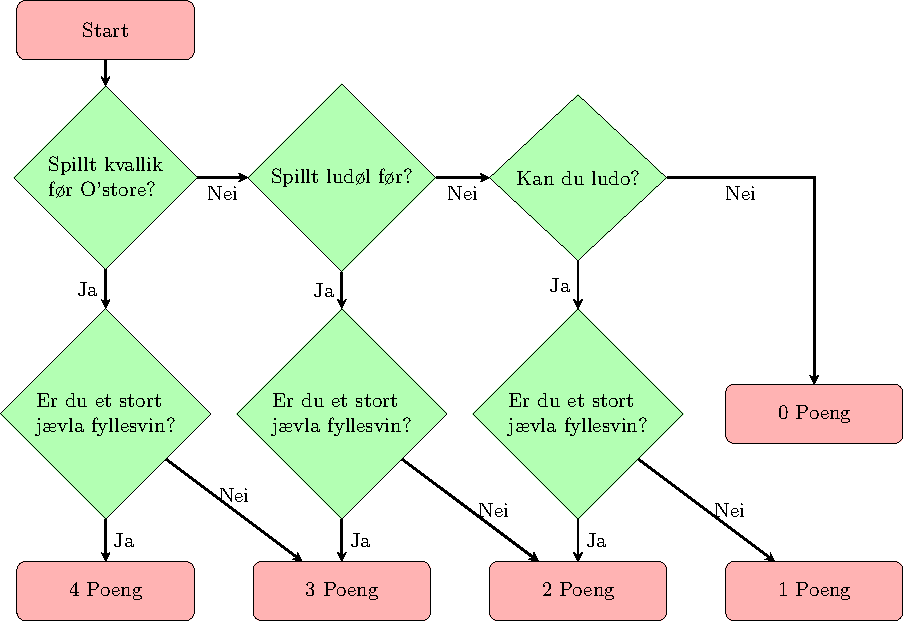
\includegraphics[width=\textwidth]{borplassering} 
  \caption{Hvordan gi poeng til deltagerne}
  \label{fig:borplassering}
\end{figure}
%
Deretter er det bare å plassere ut spilleren med høyest skåre på bordet med
lavest totalskåre, og gjenta denne prosessen til det ikke lengre er noen
spillere igjen.

\begin{figure}
  \centering
  \begin{subfigure}[b]{0.45\textwidth}
    \centering
    \bord{Indøk: 4}{Timini: 2}{Hybrida: 1}{Leonardo: 0}
    \caption{}
    \label{fig:utstyr-terning}
  \end{subfigure}
  ~ %add desired spacing between images, e. g. ~, \quad, \qquad, \hfill etc. 
  % (or a blank line to force the subfigure onto a new line)
  \begin{subfigure}[b]{0.45\textwidth}
    \centering
    \bord{Realfag: 4}{HC: 2}{Erudio: 1}{Paideia: 0}
    \caption{}
    \label{fig:utstyr-terning}
  \end{subfigure}
  
  \begin{subfigure}[b]{0.45\textwidth}
    \centering
    \bord{Omega: 4}{LaBamba: 2}{Emil: 1}{Lipton: 0}
    \caption{}
    \label{fig:utstyr-terning}
  \end{subfigure}
  ~ %add desired spacing between images, e. g. ~, \quad, \qquad, \hfill etc. 
  % (or a blank line to force the subfigure onto a new line)
  \begin{subfigure}[b]{0.45\textwidth}
    \centering
    \bord{Berg: 3}{Placebo: 2}{Nabla: 2}{Elektra: 0}
    \caption{}
    \label{fig:utstyr-terning}
  \end{subfigure}
  \caption{Eksempel på bra borplassering under O'store.}
  \label{fig:bordplassering-eksempel}
\end{figure}

Som eksempel anta at det skal spilles O'store og linjeforeningene vist i
\cref{fig:borplassering} skal delta. Tallet bak linjeforeningene er laget fra
\cref{fig:bordplassering-eksempel}. Først vil Bord 1-3 vil få Omega, Realfag og
Indøk\footnote{Selvsagt har Indøk en høy skåre. De er jo så flink å svelge}, mens
det siste bordet får Berg. Nå har Bord 4 lavest vekt, slik at de får den neste
spilleren med høyest skåre, hvor en tenker seg at Placebo ble trukket ut
tilfeldig blant alle andre spillere med skåre 2. Nå har Bord 1 lavest skåre, og
får Timini. Deretter får Bord 2 HC og Bord 3 får LaBamba. Nå står Bord 4 svakest
igjen og får Nabla som siste linjeforening. Leonardo, Paideia, Lipton og Elektra
plasseres tilslutt tilfeldig på bord 1-4.




\paragraph{Lucky Loser}

Dersom det ikke er nok deltagere til å spille med 4 bord, så velges det ofte en
``lucky looser''. De tre som vinner kommer selvsagt med i finalen, og
andreplassen som har drukket mest. Slik at en ikke kan taktisk sikkre seg en
plass i finalen.


\section{Finalen}

Mens kvalik ofte er artig, er finalen noe av det farligste en kan arrangere.
Dersom en arrangerer dette på samme kveld \emph{må} en ha edru personer klare
med bil, i tilfelle noe går galt. \textbf{Coach \emph{skal} slenge inn håndkleet
  før spillerne drikker for mye og dommer \emph{skal} være beinhard.} Aldri velg
en dommer som ikke har dømt før og husk at dersom dommer er like hard som i
kvalik går det ofte rett til helvete og sykehuset. Mens semifinalen burde vare
1-2 timer, burde finalen maks vare 1. Dommer må være en kuk av dimensjoner i
finalen slik at spillerne spyr opp alkoholen før det blir farlig. Her er noen
råd som det anbefales på det \emph{sterkeste} å følge. 

\begin{enumerate}
  \item Det er \emph{strengt} forbudt å åpne ølen for tidlig
    for å slippe ut kullsyren. Denne trengs for at deltagerne skal klare å spy.
  \item Spillerne begynner med å ta en skål i tur og orden for hver av
    spillerne i finalen
    unntatt seg selv. Med andre ord dersom Thilde, Elektra, Sukkerhuset og Lipton
    er i finalen vil da først Elektra, Sukkerhuset og Lipton få 10 sec på å ta
    en skål for Thilde. Deretter vil Thilde, Sukkerhuset, og Lipton få 10 sec på
    å ta en skål for Elektra osv. Tilslutt kan en gjerne ta en skål for
    dommeren eller arrangørene.
  \item Ingen blokkader, ingen frifelt, glassene starter ute helt fra starten.
    Viktig!
  \item Pass på å være hard på passivt spill, søling osv fra starten. Spillerne
    trenger ingen advarsler siden de allerede har spilt
  \item Innfør nye regler ca hvert 15-20 min. At spillerne får nytt kast dersom
    de slår ut noen (teller som en sekser), eller to kast per spiller er ting
    som ofte øker tempoet betraktelig. Flatrulling gitt at en drikker selv er og
    en fin regel. At blokader må flyttes som en brikke er fin å ha som siste
    spiker i kisten.
  \item Dersom spillere har muligheten å slå ut mange glass ved å trille rett,
    straff dem dersom de ikke klarer det.
  \item Alt ettersom hvordan formen er kan en og vurdere å telle ned mellom
    hvert kast. Dette er dog noe som burde informeres om ved starten av spillet.
\end{enumerate}

\chapter{Quiz}
\label{chap:quiz}
I alle disse spørsmålene kan du anta at spillet følger ``vanlige'' ludøl
regler, med de utvidelsene som er nedfelt i hus-reglene. Med andre ord
eksisterer fortsatt frifelt og blokader. I alle spørsmålene unntatt
\cref{punkt:sperrer} er det ett alternativ som er mest riktig.  

\section{Spørsmål}

\begin{enumerate}
  \item Hva er Røros-konvensjonen? 
    \begin{enumerate}
      \item At spillerne kan flytte ut av huset når det trilles én ener ($1$).
      \item At spillerne kan velge å bruke toppen, eller bunnen av terningen.
      \item At spillerne må prate med Røros-dialekt.
    \end{enumerate}
  \item Anta at spiller ikke har noen glass ute, og spiller triller $5$ hva
    skjer i følge reglene? 
    \begin{enumerate}
    \item Turen går videre til nestemann.
    \item Spiller flytter ut.
    \item Spiller triller på nytt. 
    \end{enumerate}
  \item \label{punkt:sperrer} Hvilke av alternativene sperrer i følge ludøl-reglene, og hva vil
    det si?
    \begin{enumerate}
      \item $1$ glass
      \item $2$ glass
      \item $3$ glass
      \item $4$ glass
    \end{enumerate}
  \item Anta du du spiller rød (hjerter) i \cref{fig:ludolbrett-1}. Dersom du
    triller $2$, hva er det eneste lovlige trekket du kan gjøre?
    \begin{enumerate}
      \item Flytte null ($0$) felt fremover og bli stående.
      \item Flytte et ($1$) trekk rett bak blokaden (en frem altså).
      \item Flytte to ($2$) felt fremover og slå ut blokaden
      \item Flytte to ($2$) felt fremover og stå på samme felt som blokaden
      \item Flytte fem
        ($5$) felt fremover og slå ut grønn [spar].
    \end{enumerate}
  \item Anta du spiller grønn (spar) i \cref{fig:ludolbrett-1}, ranger
    terningkastene under fra minst til mest passiv
        \begin{enumerate*}
          \item 1
          \item 2
          \item 3
    \end{enumerate*}
      \item Anta du du spiller gul (ruter) i \cref{fig:ludolbrett-1}. Hva er det
    minst passive trekket dersom du triller $5$?
    \begin{enumerate}
      \item Flytte ut av startfeltet til gul [ruter].
      \item Flytte inn i startfeltet til rød [hjerter].
      \item Bryte opp blokaden å jage blå [kløver].
    \end{enumerate}
\end{enumerate}

\begin{figure}[htbp!]
  \centering
  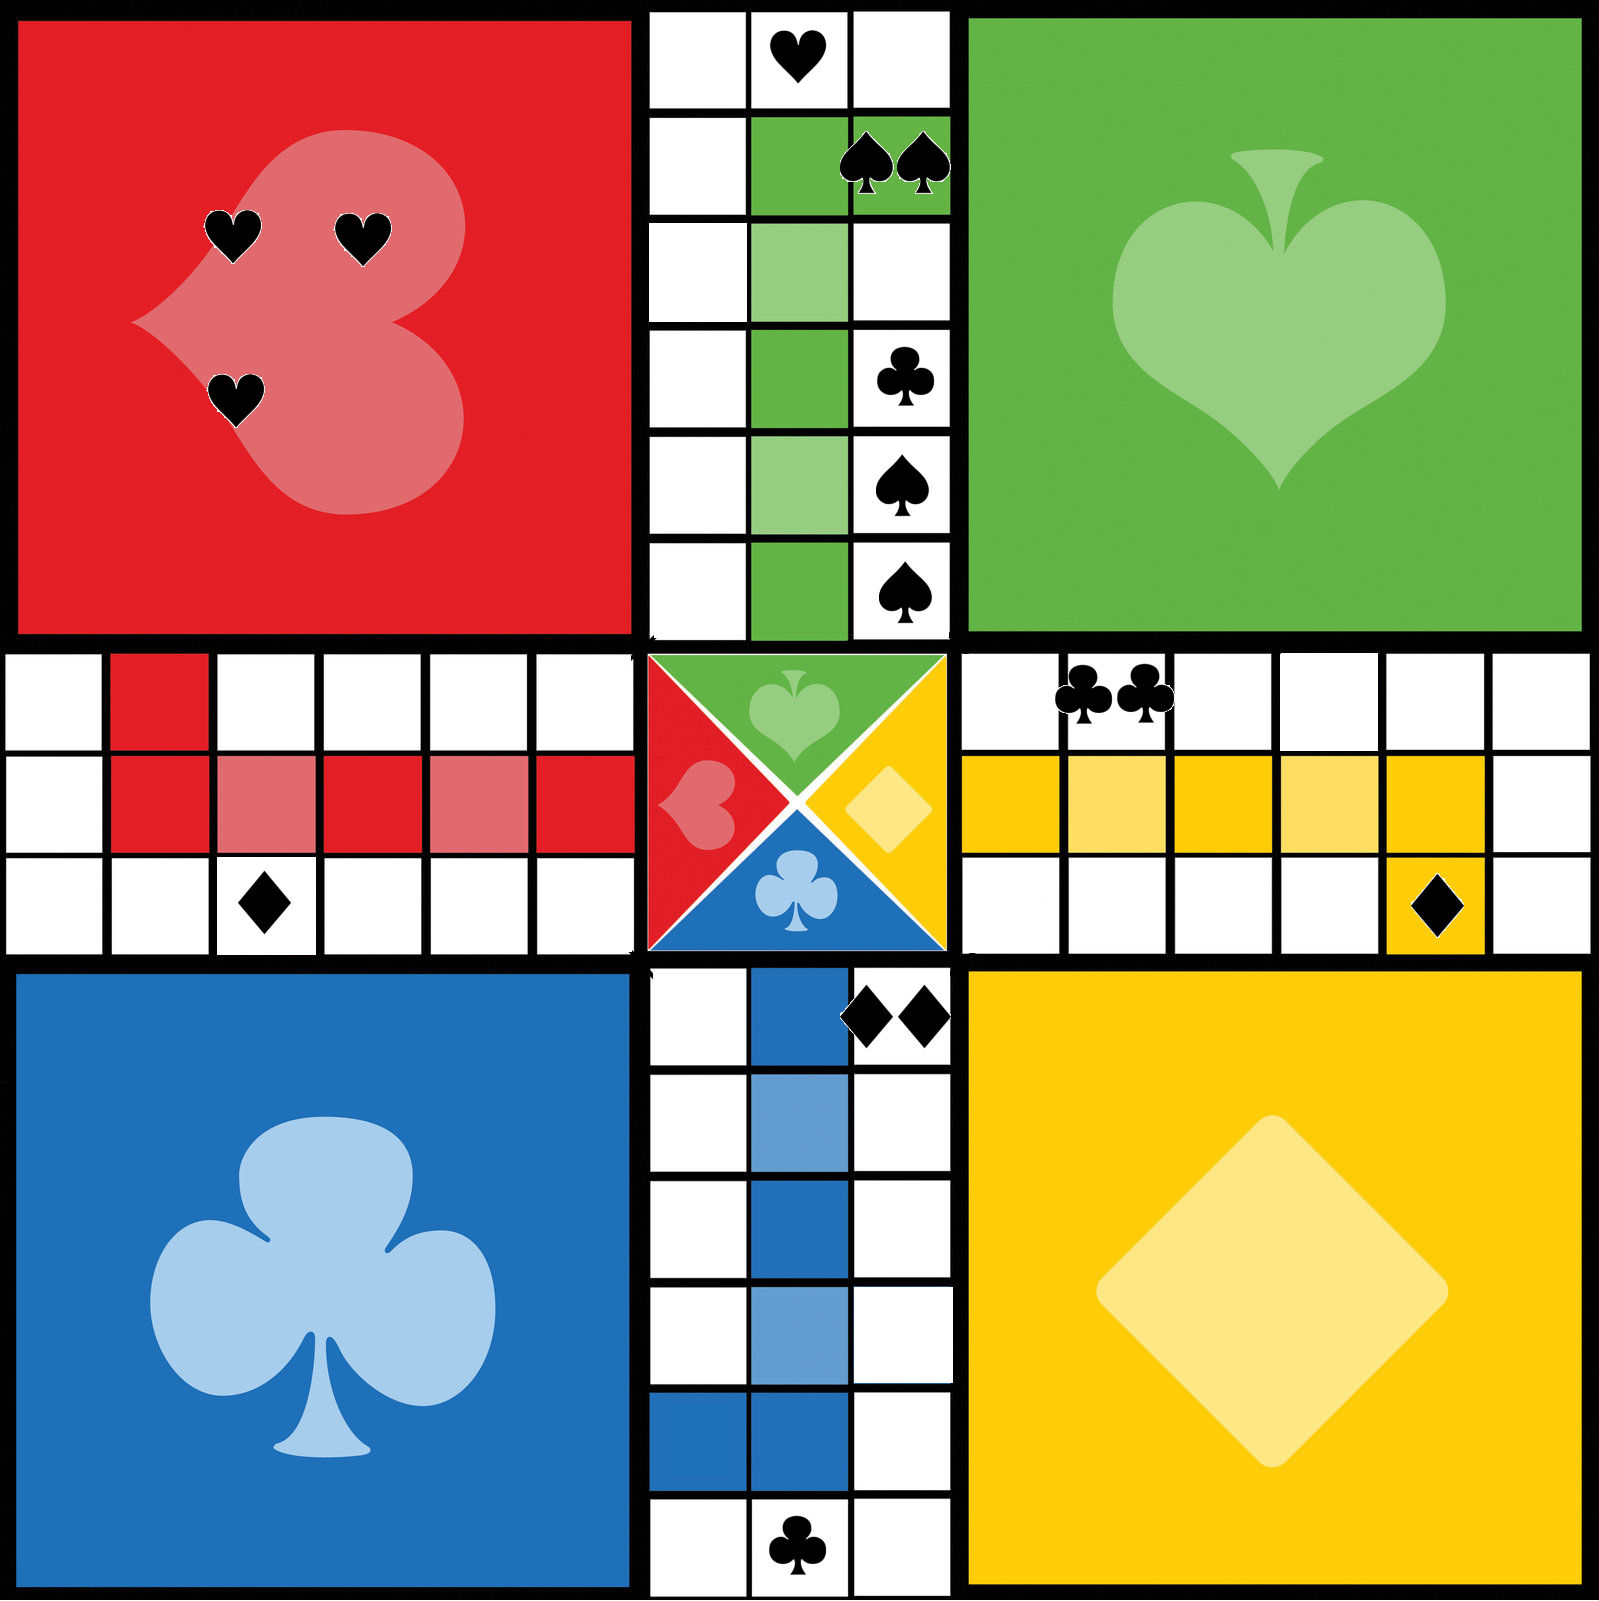
\includegraphics[width=0.5\textwidth]{ludobrett-2}
  \caption{Hypotetisk posisjon i ludøl}
  \label{fig:ludolbrett-1}
\end{figure}

\newpage

\section{Svar på quiz}

\begin{enumerate}
  \item \textbf{b)} Selv om $1$ og er riktig, følger denne fra
    Røros-konvensjonen og at en kan flytte ut dersom det trilles seks.
  \item \textbf{c)} Dersom en ikke har noen brikker ute får man $3$ forsøk på
    å komme seg ut av huset.
  \item \textbf{b)} og \textbf{d)}. At $2$ og $4$ glass sperrer betyr at
    det ikke er mulig å flytte forbi disse glassene, eller slå dem ut.
  \item \textbf{a)} Presisering av forrige spørsmål, det er i utgangspunktet
    ikke lov å flytte dersom det eksisterer en blokade foran seg.
  \item \textbf{b)}, \textbf{a)}, \textbf{c)}. Anta at en triller seks ($6$).
    Siden alle glassene står ute og det eksisterer en blokade foran, kan en ikke
    velge $(6)$ men må velge
    $1$. En har da muligheten til enten å lage en blokade, eller flytte til et
    tomt felt. Det å flytte en frem er passivt, men ikke like passivt som å
    skape en blokade.

    Dersom det trilles to ($2$) kan en slå ut blå (kløver), eller flytte til et
    tomt felt. Åpenbart burde en her slå ut blå.

    Dersom det trilles tre ($3$), skaper man en blokade enten en velger tre
    ($3$) eller ($4$) på terningen. Dette er det mest passive trekket.
  \item \textbf{b)}. Uavhengig av hvilke glass gul [ruter] velger å flytte,
    er det passivt å flytte $2$. Dermed bør en flytte ett av glassene $5$
    frem mover. La oss ta for oss hvert av alternativene.

    Dersom en flytter glasset som står i gult frifelt fem ($5$) felt fremover
    så flytter ut av frifeltet og en bryter opp blokaden siden tre
    glass ikke sperrer. Men, det er ingen andre spillere som står nærme nok til
    å kunne angripe disse tre glassene. Dette trekket er med andre ord ikke
    spesielt aggressivt

    Det er heller ingen grunn til å jage blå (kløver). Kløver har en blokade
    oppe i høyre hjørnet, og det vil være lurt å bryte opp denne før en flytter
    glasset i nede i venstre hjørnet. Dermed kan en slå ut kløver neste runde
    ved å trille seks ($6$). Dersom en flytter frem rett bak blå
    (kløver) måtte en ha valgt en ($1$) på terningen neste runde for å slå ut.
    Med andre ord tjener man ett ekstrakast ved å ikke flytte frem.

    Det å flytte inn i startfeltet til rød er det mest aggressive trekket en kan
    gjøre. Spesielt siden rød bare har en brikke ute på brettet.
  \item 
\end{enumerate}

\end{document}